I% Chapter Template

\chapter{Optimizations} % Main chapter title

\label{Optimizations} % Change X to a consecutive number; for referencing this chapter elsewhere, use \ref{ChapterX}

\lhead{Optimizations. \emph{Optimizations}} % Change X to a consecutive number; this is for the header on each page - perhaps a shortened title

%----------------------------------------------------------------------------------------
%	SECTION - Where does time go?
%----------------------------------------------------------------------------------------

\section{Where is time spent?}

%-----------------------------------
%	SUBSECTION 1
%-----------------------------------

\subsection{Arrays}
% array creation, copy
Most of the memory used in the vector data structure is composed of arrays. The three key operations used on these arrays: array creation, array update and array access. The arrays are used as immutable arrays, as such the update operations are only allowed when the array is initialised. This also implies that each time there is a modification on some part of an array, a new array must be created and all the old elements copied. 

% size of array argument
The size of the array will affect the performance of the vector. With larger blocks the access times will be reduced because the depth of the tree will decrease. But, on the other hand, increasing the size of the block will make slow down the update operations. This is a direct consequence of the need to copy the entire array for a single update.


%-----------------------------------
%	SUBSECTION 2
%-----------------------------------

\subsection{Computing indices}
\label{ComputingIndices}

Computing the indices in each node while traversing or modifying the vector is key in performance. This performances is gained by using low level binary computations on the indices in the case where the tree is balanced. And, using precomputed sizes in the case where the balance is relaxed.

%-----------------------------------
\paragraph{Radix}
% Explain how to compute them
Assuming that the tree is full, elements are fetched from the tree using radix search on the index. As each node has a branching of 32, the index can be split bitwise in blocks of 5 ($2^5 = 32$) and used to know the path that must be taken from the root down to the element. The indices at each level $L$ can be computed with $(index >> (5 \cdot L)) \& 31$. For example the index 526843 would be:
\[
 526843 = 00
   	 \underbracket[0.2pt][4pt]{00000}_{\text{0}}
   	 \underbracket[0.2pt][4pt]{00000}_{\text{0}}
  	 \underbracket[0.2pt][4pt]{10000}_{\text{16}}
 	 \underbracket[0.2pt][4pt]{00010}_{\text{2}}
	 \underbracket[0.2pt][4pt]{01111}_{\text{15}}
     \underbracket[0.2pt][4pt]{11011}_{\text{27}}
\]

\begin{lstlisting}[frame=single]
def getSubIndex(indexInTree: Int, level: Int): Int = 
  (index >> (5*level)) & 31
\end{lstlisting}

% how to generalise
This scheme can be generalised to any block size $m$ where $m=2^i$ for $0 < i \leq 31$. The formula would be $(index >> (m \cdot L)) \& ((1<<m)-1)$. It is also possible to generalise for other values of $m$ using the modulo, division and power operations. In that case the formula would become $(index / (m^L)) \% m$. This last generalisation is not used because it reduces sightly the performance and it complicates other index manipulations. 

\begin{figure}[h!]
  \centering
  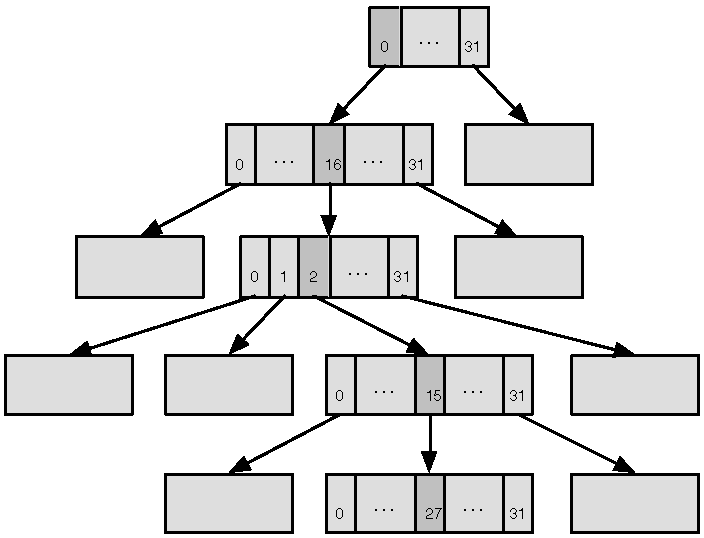
\includegraphics[width=0.5\textwidth]{Figures/Radix_Balanced_index_example}
  \caption{Accessing element at index 526843 in a tree of depth 5. Empty nodes represent collapses subtrees.}
  \label{radix_balanced_index_example}
\end{figure}

%-----------------------------------
\paragraph{Relaxing the Radix}
% Explain how to compute them 
When the tree is relaxed it is not possible to know the subindices from index. That is why we keep the sizes array in the unbalanced nodes. This array keeps the accumulated sizes to make the computation of subindices as trivial as possible. The subindex is the same as the first index in the sizes array where $index < sizes[subindex]$. The simplest way to find this subindex is by a linearly scanning the array. 

\begin{lstlisting}[frame=single]
def getSubIndex(sizes: Array[Int], indexInTree: Int): Int = {
  var is = 0
  while (sizes(is) <= indexInTree)
    is += 1
  is
}
\end{lstlisting}

% linear vs binary search
For small arrays (like blocks of size 32) this will take be faster than a binary search because it takes advantage of the cache lines. If we would consider using bigger block sizes it would be better to use a hybrid between binary and linear search.

% fallback to radix
To traverse the tree down to the leaf where the index is, the subindices are computed from the sizes as long as the tree node is unbalanced. If the node is balanced, then the more efficient radix based method is used from there to the leaf. To avoid the need of accessing and scanning an additional array in each level.


%-----------------------------------
%	SUBSECTION 3
%-----------------------------------

\subsection{Abstractions}
% function calls
% generic code vs specialized code
% expanded code 
% example with simple expanded get operation (show expansion and specialisation)


%----------------------------------------------------------------------------------------
%	SECTION - Displays
%----------------------------------------------------------------------------------------

\section{Displays}
\label{sec:Displays}
% describe display fields in vector object
As base for optimizations, the vector object keeps a set of fields to track one branch of the tree. They are named with using the level number from 0 up to the maximum possible level. In the case of blocks of size 32 the maximum level used is 5 \footnote{As in practice, only the 30 bits of the index are used.}, they are allocated by default and nulled if the tree if shallower. The highest non null display is and replaces the root field. All displays bellow the root are never null. This implies that the vector will always be focused on some branch.

\begin{figure}[h!]
  \centering
  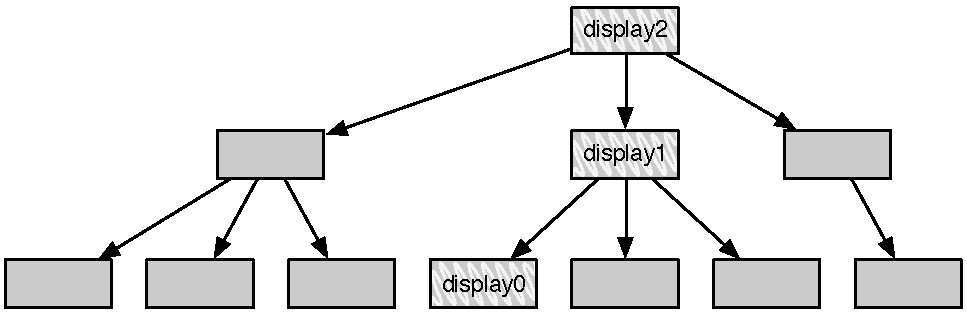
\includegraphics[width=0.8\textwidth]{Figures/Displays}
  \label{Displays}
  \caption{Displays}
\end{figure}

% describe the focus field
To know on which branch the vector is focused there is also a \texttt{focus} field with an index. This index is the index of any element in the current \texttt{display0}. This index represents the radix indexing scheme of node subindices described in \ref{ComputingIndices}.

% immutability of displays
To follow the simple implementations scheme of immutable objects in concurrent contexts, the focus is also immutable. Therefore each vector object will have a single focused branch during its existence\footnote{The display focus may change during the initialisation of the object as optimisation of some methods}. Each method that creates a new vector must decide which focus to set. 

%-----------------------------------
%	SUBSECTION As cache
%-----------------------------------

\subsection{As cache}
% used to access some elements directly from the smaller subtrees (XOR)
One of the uses of the displays is as a cached branch. If the same leaf node is used in the following operation, there is no need for vertical tree traversal which is key to amortize operation to constant time. In the case another branch in needed, then it can be fetched from the lowest common node of the two branches. 

% xor
To know the which is the level of the lowest common node in a vector of block size $2^m$ (for some consistent $m$), only the \texttt{focus} index and the index being fetched are needed. The operation $index \veebar focus$ will return a number is bounded to the maximum number of elements in a tree of that level. The actual level can be extracted with some if statements. This operation bounded by the same number of operations that will be needed to traverse the tree back down through the new branch.

\begin{lstlisting}[frame=single]
def getLowestCommonLevel(index: Int, focus: Int): Int = {
  val xor = index ^ focus
  if (xor < 32 /*(1<<5)*/ ) 0
  else if (xor < 1024 /*(1<<10)*/ ) 1
  else if (xor < 32768 /*(1<<15)*/ ) 2
  ...
  else 5
}
\end{lstlisting}

% keeping relevant branch for next operations
When deciding which will be the focused branch of a new vector two heuristics are used for this: If there was an update operation on some branch where that operations could be used again, that branch is used as focus. If the first one cant be applied, the display is set to the first element as this helps key collection operations such as \texttt{iterator}.

%-----------------------------------
%	SUBSECTION  For transient states
%-----------------------------------

\subsection{For transient states}
% operation: append, prepend, update
Transient states is the key optimisation to get append, prepend and update to amortized constant time. It consists in decoupling the tree by creating an equivalent tree that does not contain the edges on the current focused branch. The information missing in the edges of the tree is represented and can be reconstructed from the displays. In the current version of the collections vector \cite{scalaVector211} this state is identified by the \texttt{dirty} flag.

\begin{figure}[h!]
  \centering
  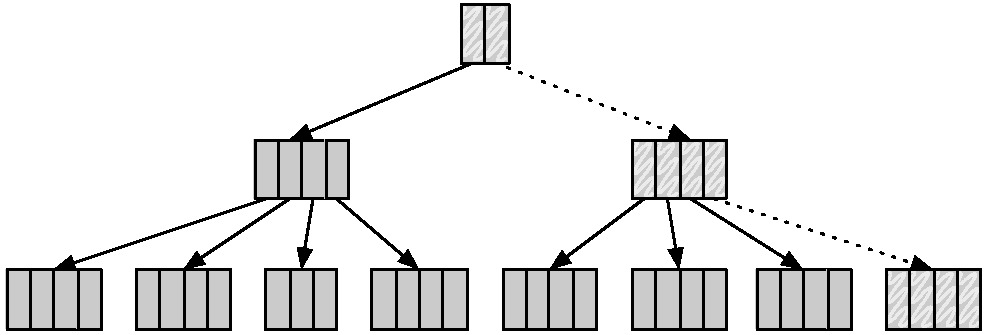
\includegraphics[width=\textwidth]{Figures/Transient_state}
  \label{Transient_state}
  \caption{Transient Tree with current focus displays marked in white and striped nulled edges.}
\end{figure}

% transient states are used to amortized operations
Without transient states when some update is done on a leaf, all the branch must be updated. On the other hand, if the state is transient, it is possible to update only the subtree affected by the change. In the case of updates on the same leaf, only the leaf must be updated. When appending or prepending, $\frac{31}{32}$ operations must only update the leaf, then $\frac{31}{1024}$ need to update two levels of the tree and so on. These operations will thus be amortized to constant ($\sum_{k=1}^{\infty} \frac{k*31}{32^k} = \frac{32}{31}$ block updates per operation) time if they are executed in succession.

% normailization
There is a cost associated to the transformation from normal state to transient state and back. This cost is equivalent to one update of the focused branch. The transient state operations only start gaining performance on the normal ones after 3 consecutive operations. With 2 consecutive operations they are matched and with 1 there is a loss of performance.


%-----------------------------------
%	SUBSECTION  Relaxing the Displays
%-----------------------------------

\subsection{Relaxing the Displays}
% describe fundamental difference in the focus (focused on balanced subtree)
When relaxing the tree balance it is also necessary to relax the displays. This is mainly due to the loss of a simple way to compute the lowest common node on unbalanced trees. Computing the node requires now the additional sizes information located in each unbalanced node. As such it is necessary to access the nodes to be abel to compute the lowest common node, and there is a loss in performance due to increased memory accesses. 

% describe focus start, focus end and focus (focus relaxed)
To still take advantage of efficient operations on balanced trees, the display is relaxed to be focused on a branch of some balanced subtree\footnote{A fully balanced tree will be itself the balanced subtree, as such it will always use the more performant operations.}. To keep track of this subtree there are three additional fields: \texttt{focusStart} that represents start index of the current focused subtree, \texttt{focusEnd} that represents the end index of the subtree and \texttt{focusDepth} that sets  height of the focused subtree\footnote{As an optimisation, the \texttt{focus} field is split into the part corresponding to the subtree and the part that represents the indices of the displays that are unbalanced.}. The operations that can take advantage of the the efficient display operations will check if the index is in the subtree index range and invoke the efficient operation. If not, it will invoke the relaxed version of the operation, that starts from the root of the tree.

% describe how fetching elements change
For example, the code for \texttt{getElement} would become:
\begin{lstlisting}[frame=single]
def getElement(index: Int): A = {
  if (focusStart <= index && index < focusEnd) 
    getElementFromDisplay(index - focusStart)
  else if (0 <= index && index < endIndex) 
    getElementFromRoot(index)    
  else 
    throw new IndexOutOfBoundsException(index)
}
\end{lstlisting}

This \texttt{getElement} on the unbalanced subtrees of figure \ref{Balanced_subtrees}  would use the \texttt{getElementFromDisplay} to fetch elements in \texttt{display0} directly from it and fetch elements from nodes (1.1) and (1.2) from \texttt{display1}. The rest is fetched from the root using \texttt{getElementFromRoot}.

\begin{figure}[h!]
  \centering
  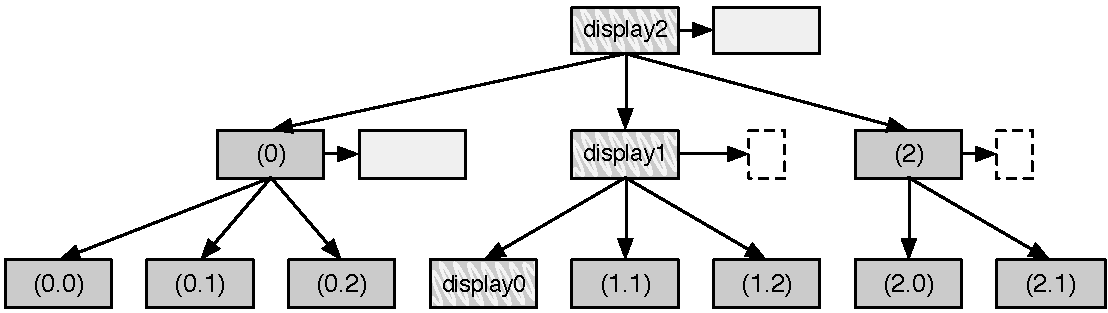
\includegraphics[width=\textwidth]{Figures/Balanced_subtrees}
  \caption{Relaxed Radix Balanced Tree with a focus on a balanced subtree rooted of \texttt{display1}. Light grey boxes represent unbalanced nodes sizes.}
  \label{Balanced_subtrees}
\end{figure}


%----------------------------------------------------------------------------------------
%	SECTION - Builder
%----------------------------------------------------------------------------------------

\section{Builder}
% use of mutable tree 
% avoid creation unnecessary arrays


%-----------------------------------
\paragraph{Relaxing the Builder}
% same base implementation for +=
% addition of accumulator for  ++= 



%----------------------------------------------------------------------------------------
%	SECTION - Iterator
%----------------------------------------------------------------------------------------

\section{Iterator}
% efficient tree traversal vs iteration by index
% avoid re-traversing vertically the tree from the root

%-----------------------------------
\paragraph{Relaxing the Iterator}
% same implementation within a balanced subtree
% refocus from root to iterate between balanced subtrees







